% TO-DO:
% * slides to mention big achievements, 附件

\documentclass[16pt]{beamer}

\ifdefined\chinchin
\usepackage[CJKspace]{xeCJK}
%\setCJKmainfont[BoldFont=SimHei,ItalicFont=AR PL KaitiM GB]{Alibaba PuHuiTi}
\setCJKmainfont{Alibaba PuHuiTi}
\newcommand{\cc}[2]{#1}
\else
\newcommand{\cc}[2]{#2}
\renewcommand{\baselinestretch}{0.8} 
\fi

%\usepackage{newtxtext,newtxmath}	% use Times Roman font
%\usepackage{newtxtext}
%\renewcommand{\familydefault}{\sfdefault}
\usefonttheme{serif}
\usefonttheme{professionalfonts}
%\setbeamertemplate{theorems}[numbered]
\setbeamertemplate{caption}{\insertcaption} 	% no `Figure' prefix before caption

\mode<presentation> {

%\usetheme{default}
%\usetheme{AnnArbor}
%\usetheme{Antibes}
%\usetheme{Bergen}
%\usetheme{Berkeley}
%\usetheme{Berlin}
%\usetheme{Boadilla}
%\usetheme{CambridgeUS}
%\usetheme{Copenhagen}
%\usetheme{Darmstadt}
%\usetheme{Dresden}
%\usetheme{Frankfurt}
%\usetheme{Goettingen}
%\usetheme{Hannover}
%\usetheme{Ilmenau}
%\usetheme{JuanLesPins}
%\usetheme{Luebeck}
\usetheme{Madrid}
%\usetheme{Malmoe}
%\usetheme{Marburg}
%\usetheme{Montpellier}
%\usetheme{PaloAlto}
%\usetheme{Pittsburgh}
%\usetheme{Rochester}
%\usetheme{Singapore}
%\usetheme{Szeged}
%\usetheme{Warsaw}

%\usecolortheme{albatross}
%\usecolortheme{beaver}
%\usecolortheme{beetle}
%\usecolortheme{crane}
%\usecolortheme{dolphin}
%\usecolortheme{dove}
%\usecolortheme{fly}
%\usecolortheme{lily}
\usecolortheme{orchid}
%\usecolortheme{rose}
%\usecolortheme{seagull}
%\usecolortheme{seahorse}
%\usecolortheme{whale}
%\usecolortheme{wolverine}		% Hofstra

%\setbeamertemplate{footline} % To remove the footer line in all slides uncomment this line
\setbeamertemplate{footline}[page number] % To replace the footer line in all slides with a simple slide count uncomment this line
\setbeamertemplate{navigation symbols}{} % To remove the navigation symbols from the bottom of all slides uncomment this line
}

\setbeamertemplate{headline}{}
% \setbeamersize{text margin left=1mm,text margin right=1mm} 
% \settowidth{\leftmargini}{\usebeamertemplate{itemize item}}
% \addtolength{\leftmargini}{\labelsep}
% \setbeamertemplate{enumerate subitem}{(\roman{enumii})}
% \setbeamertemplate{itemize items}[default]
\setbeamertemplate{items}[square]
\setbeamertemplate{enumerate items}[default]

\usepackage[backend=biber,style=numeric]{biblatex}
\bibliography{../AGI-book}
% \renewcommand*{\bibfont}{\footnotesize}
\setbeamertemplate{bibliography item}[text]

\usepackage{graphicx} % Allows including images
\usepackage{tikz-cd}
\usepackage{tikz}
\usepackage[export]{adjustbox}% http://ctan.org/pkg/adjustbox
\usepackage{verbatim} % comments
\usepackage[skins,theorems]{tcolorbox}

\usepackage{ulem}
\makeatletter
\newcommand{\cthickuline}[3][0.5pt]{%
	\UL@protected\def\temp@uline{\bgroup\markoverwith
		{\textcolor{#2}{\rule[-0.5ex]{2pt}{#1}}}\ULon}%
	\temp@uline{#3}%
}
\makeatother

% \usepackage{tikz-cd}  % commutative diagrams
% \newcommand{\tikzmark}[1]{\tikz[overlay,remember picture] \node (#1) {};}
% \usepackage{booktabs} % Allows the use of \toprule, \midrule and \bottomrule in tables
% \usepackage{amssymb}  % \leftrightharpoons
% \usepackage{wasysym} % frownie face
% \usepackage{newtxtext,newtxmath}	% Times New Roman font
% \usepackage{sansmath}

\newcommand{\emp}[1]{\textbf{\color{violet}#1}}
\newcommand{\vect}[1]{\boldsymbol{#1}}
\newcommand{\tab}{\hspace*{1cm}}
\newcommand*\confoundFace{$\vcenter{\hbox{\includegraphics[scale=0.2]{../confounded-face.jpg}}}$}
\newcommand{\smiley}{$\vcenter{\hbox{\includegraphics[scale=0.05]{../smiling-face.png}}}$}

\makeatletter
\renewcommand{\boxed}[1]{\fbox{\m@th$\displaystyle\scalebox{0.9}{#1}$} \,}
\makeatother

%----------------------------------------------------------------------------------------
%	TITLE PAGE
%----------------------------------------------------------------------------------------

\title[AGI and categorical logic]{{Paper: AGI from the perspectives of categorical logic and algebraic geometry}}
\author{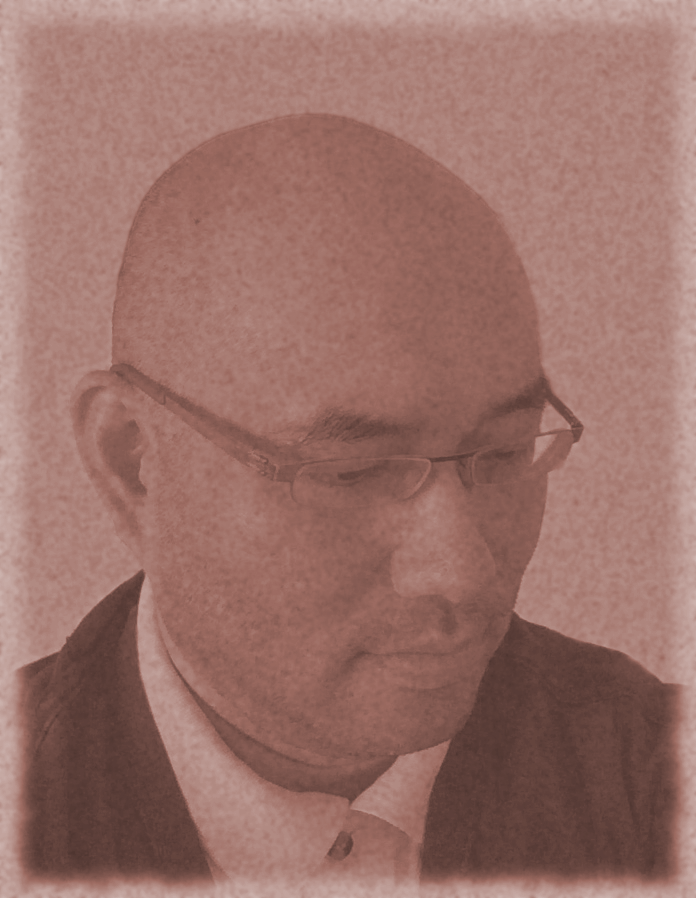
\includegraphics[scale=0.14]{John_Grothendieck.png} \\ \centering YKY}
\date{\today} % Date, can be changed to a custom date

\begin{document}

\addtocounter{page}{-1}
\begin{frame}[plain,noframenumbering]
\titlepage
\end{frame}

\addtocounter{page}{-1}
\begin{frame}[noframenumbering]
\frametitle{Contents}
\tableofcontents
% \vspace*{0.5cm}
% 多谢 支持 \smiley
\end{frame}

%----------------------------------------------------------------------------------------
%	PRESENTATION SLIDES
%----------------------------------------------------------------------------------------

\section{How does ``No Free Lunch'' guide us to accelerate AGI?}
\subsection{The hypothesis space}
\subsection{A motivating example of mapping spaces}
\subsection{Dumb animals and dumb knowledge}
\section{Basics of categorical logic}
\section{Fibrations in particular}

\part{How does ``No Free Lunch'' guide us to accelerate AGI?}
\frame{\partpage}

\begin{frame}
\frametitle{The hypothesis space}

In deep learning, our hypothesis space = neural networks = parameter space = weight space = $\mathbb{R}^n$ or $[0,1]^n$.

It looks like this:
\begin{equation}
\vcenter{\hbox{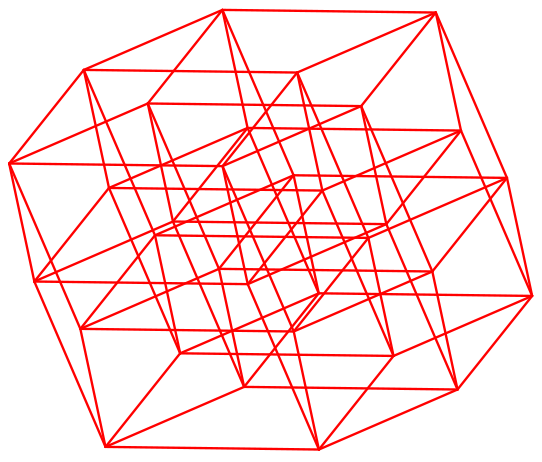
\includegraphics[scale=0.3]{hypercube.png}}}
\nonumber
\end{equation}

Imagine a loss function as sitting above this space;  We seek to minimize it by gradient descent.
\end{frame}

\begin{frame}
\frametitle{The hypothesis space has plenty of ``dumb structures''}
\centering
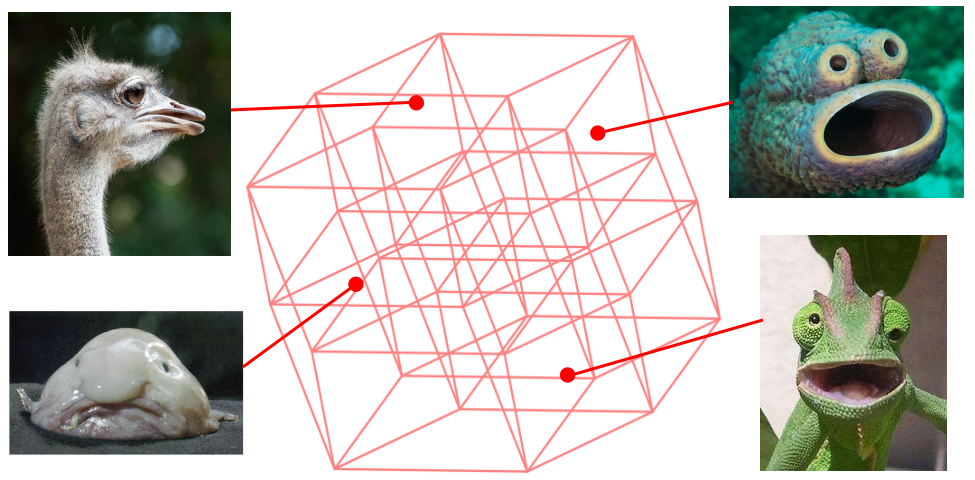
\includegraphics[scale=0.35]{dumb.png}
\vspace*{1em}
\begin{itemize}
	\item Nature has produced more dumb animals than intelligent ones
\end{itemize}
\end{frame}

\part{Basics of categorical logic}
\frame{\partpage}

\begin{frame}
\frametitle{Curry-Howard isomorphism}
\begin{itemize}
	\item ``Floating'' regions and points as models
\end{itemize}
\end{frame}

\part{Fibrations in particular}
\frame{\partpage}

\begin{frame}
\frametitle{Definition of a \textbf{fiber bundle}}
A \textbf{fiber bundle} is a tuple $\xi = (E, p, B, F)$ such that:
\begin{enumerate}[(i)]
	\item $E$ = \textbf{total space}
	\item $B$ = \textbf{base space}
	\item $F$ = a topological space called the \textbf{fiber} of $\xi$
	\item $\mathrel{\substack{E\\\downarrow \\B}  {\scriptstyle p}}$ is a continuous surjective map, called the \textbf{projection}
	\item for each point $b \in B$, the inverse image $p^{-1}(b) = F_b$, called \cthickuline[1.2pt]{red}{the \textbf{fiber over} $b$, is homeomorphic to $F$}
	\item $B$ has an opening covering $\{ U_a \}_{a \in A}$ such that for each $a \in A$, there is a homeomorphism: $\psi_a: U_a \times F \rightarrow p^{-1}(U_a)$.  \\
	If $F$ is a discrete space, then the structure $F \hookrightarrow E \stackrel{p}{\rightarrow} B$ is called a \textbf{covering} of $B$.
\end{enumerate}

The condition (vi) is just a re-phrase of (v) in the form of open sets, similar to the ``gluing'' together of charts in differential manifolds.  So the essential condition is (v).

\end{frame}

\begin{frame}
\frametitle{The ``boring'' cross product}

\begin{equation}
	\tcbhighmath[boxrule=1pt,arc=6pt,colframe=black,shrink tight,extrude by=2mm]{token} \qquad
	\tcbhighmath[boxrule=1pt,arc=6pt,colframe=black,shrink tight,extrude by=2mm]{token} \qquad
	\tcbhighmath[boxrule=1pt,arc=6pt,colframe=black,shrink tight,extrude by=2mm]{token}
	\nonumber
\end{equation}
is equivalent to $A \times A \times A$.

\end{frame}


\begin{frame}
\frametitle{References}
\cc{多谢收看}{Thanks for watching} \smiley \\
% \printbibliography
\end{frame}

\end{document} 